\documentclass{article}

% content/resources/templates/preamble.tex
\usepackage[margin=0.6in]{geometry}
\author{Milav Dabgar}
\usepackage{amsmath,amssymb,amsthm}
\usepackage{booktabs}
\usepackage{multirow}
\usepackage{xcolor}
\usepackage{tcolorbox}
\tcbuselibrary{breakable,skins}
\usepackage[colorlinks=true,linkcolor=blue]{hyperref}
\usepackage{titlesec}
\usepackage{enumitem}
\usepackage{tikz}
\usepackage{pgfplots}
\usepackage{circuitikz}
\usepackage[version=4]{mhchem}
\usepackage{longtable}
\usepackage{array}
\usepackage{float}
\usepackage{caption}
\usepackage{listings}

\lstset{
  basicstyle=\small\ttfamily,
  breaklines=true,
  breakatwhitespace=false,
  postbreak=\mbox{\textcolor{red}{$\hookrightarrow$}\space},
  float=false,
  numbers=left,
  numberstyle=\tiny\color{gray},
  numbersep=10pt,
  xleftmargin=2em,
  keywordstyle=\color{blue},
  commentstyle=\color{green!60!black},
  stringstyle=\color{purple},
  backgroundcolor=\color{gray!5},
  showstringspaces=false,
  tabsize=2,
  captionpos=b,
  keepspaces=true,
  columns=flexible
}

\pgfplotsset{compat=1.18}
\usetikzlibrary{shapes,arrows,positioning,calc,patterns,decorations.pathmorphing,decorations.markings,arrows.meta}

% Color scheme
\definecolor{headcolor}{RGB}{0,102,204}
\definecolor{keycolor}{RGB}{220,20,60}
\definecolor{solutioncolor}{RGB}{34,139,34}
\definecolor{mnemoniccolor}{RGB}{148,0,211}
\definecolor{codecolor}{RGB}{0,0,100}

% Spacing
\setlength{\parskip}{3pt}
\setlist[itemize]{nosep}
\setlist[enumerate]{nosep}

% Title formatting
\titleformat{\section}{\Large\bfseries\color{headcolor}}{\thesection}{1em}{}
\titleformat{\subsection}{\large\bfseries\color{headcolor}}{\thesubsection}{1em}{}

% Pandoc tightlist compatibility
\providecommand{\tightlist}{%
  \setlength{\itemsep}{0pt}\setlength{\parskip}{0pt}}

% Pandoc longtable compatibility
\newcounter{none}
\def\thenone{}


% content/resources/templates/english-boxes.tex

% Custom environments
\newtcolorbox{solutionbox}{
 breakable,
 enhanced,
 colback=solutioncolor!5!white,
 colframe=solutioncolor!75!black,
 fonttitle=\bfseries,
 title=Solution
}

\newtcolorbox{solutionboxnobreak}{
 colback=solutioncolor!5!white,
 colframe=solutioncolor!75!black,
 fonttitle=\bfseries,
 title=Solution
}

\newtcolorbox{keyformula}{
 breakable,
 enhanced,
 colback=keycolor!5!white,
 colframe=keycolor!75!black,
 fonttitle=\bfseries,
 title=Key Formula
}

\newtcolorbox{mnemonicboxenv}{
 breakable,
 enhanced,
 colback=mnemoniccolor!5!white,
 colframe=mnemoniccolor!75!black,
 fonttitle=\bfseries,
 title=Mnemonic
}

\newcommand{\mnemonicbox}[1]{%
  \begin{mnemonicboxenv}
    #1
  \end{mnemonicboxenv}
}


% Custom commands for GTU solutions
% This file defines semantic commands for consistent formatting

% Question command with automatic formatting
\newcommand{\question}[2]{%
  \section*{Question #1}%
  \textbf{#2}%
}

% OR question variant
\newcommand{\questionor}[2]{%
  \section*{Question #1 OR}%
  \textbf{#2}%
}

% Proper table environment with caption
\newenvironment{answertable}[1]{%
  \begin{table}[htbp]
  \centering
  \caption{#1}
}{%
  \end{table}
}

% Proper figure environment for diagrams
\newenvironment{answerdiagram}[1]{%
  \begin{figure}[htbp]
  \centering
  \caption{#1}
}{%
  \end{figure}
}

% Semantic markup for key terms
\newcommand{\keyword}[1]{\textbf{#1}}
\newcommand{\code}[1]{\texttt{#1}}
\newcommand{\classname}[1]{\texttt{#1}}
\newcommand{\methodname}[1]{\texttt{#1}}

% Proper quotation marks
\newcommand{\mnemonic}[1]{``#1''}


\usetikzlibrary{fit}

\title{Software Engineering (4353202) - Winter 2024 Solution}
\date{November 25, 2024}

\begin{document}
\maketitle

\questionmarks{1(a)}{3}{Define software and explain its characteristics.}

\begin{solutionbox}
\textbf{Software} is a collection of computer programs, procedures, and documentation that performs tasks on a computer system.

\begin{center}
\captionof{table}{Software Characteristics}
\begin{tabulary}{\linewidth}{|L|L|}
\hline
\textbf{Characteristic} & \textbf{Description} \\ \hline
\textbf{Intangible} & Cannot be touched, only experienced \\ \hline
\textbf{Developed} & Engineered, not manufactured \\ \hline
\textbf{Maintainable} & Can be modified and updated \\ \hline
\textbf{Reliable} & Should work consistently \\ \hline
\textbf{Efficient} & Uses resources optimally \\ \hline
\end{tabulary}
\end{center}

\begin{itemize}
    \item \textbf{Key point}: Software = Programs + Documentation + Procedures
\end{itemize}
\end{solutionbox}

\begin{mnemonicbox}
\mnemonic{I Don't Make Reliable Electronics (Intangible, Developed, Maintainable, Reliable, Efficient)}
\end{mnemonicbox}

\questionmarks{1(b)}{4}{Explain classical waterfall model.}

\begin{solutionbox}
\textbf{Waterfall Model} is a linear sequential software development approach where each phase must be completed before the next begins.

\begin{center}
\begin{tikzpicture}[node distance=1.5cm, auto]
    \node [gtu block] (req) {Requirements Analysis};
    \node [gtu block, below of=req] (des) {System Design};
    \node [gtu block, below of=des] (impl) {Implementation};
    \node [gtu block, below of=impl] (test) {Testing};
    \node [gtu block, below of=test] (dep) {Deployment};
    \node [gtu block, below of=dep] (maint) {Maintenance};

    \draw [gtu arrow] (req) -- (des);
    \draw [gtu arrow] (des) -- (impl);
    \draw [gtu arrow] (impl) -- (test);
    \draw [gtu arrow] (test) -- (dep);
    \draw [gtu arrow] (dep) -- (maint);
\end{tikzpicture}
\captionof{figure}{Classical Waterfall Model}
\end{center}

\textbf{Key Features}:
\begin{itemize}
    \item \textbf{Sequential phases}: No overlap between phases
    \item \textbf{Documentation-driven}: Heavy documentation at each phase
    \item \textbf{Simple structure}: Easy to understand and manage
    \item \textbf{Fixed requirements}: Changes are difficult once started
\end{itemize}
\end{solutionbox}

\begin{mnemonicbox}
\mnemonic{Real Systems Include Testing, Deployment, Maintenance}
\end{mnemonicbox}

\questionmarks{1(c)}{7}{Explain software process framework and umbrella activities.}

\begin{solutionbox}
\textbf{Software Process Framework} provides the foundation for complete software engineering process by identifying key process areas.

\begin{center}
\begin{tikzpicture}[node distance=2cm, auto]
    % Framework Activities in a cycle
    \node [gtu state] (comm) {Communication};
    \node [gtu state, right of=comm] (plan) {Planning};
    \node [gtu state, right of=plan] (model) {Modeling};
    \node [gtu state, right of=model] (const) {Construction};
    \node [gtu state, right of=const] (dep) {Deployment};

    \path [gtu arrow] (comm) -- (plan);
    \path [gtu arrow] (plan) -- (model);
    \path [gtu arrow] (model) -- (const);
    \path [gtu arrow] (const) -- (dep);
    \path [gtu arrow] (dep) edge [bend left=30] (comm);
    
    % Umbrella Activities spanning across
    \node [draw, headcolor, dashed, fit=(comm) (dep), inner sep=1cm, label=above:\textbf{Umbrella Activities}] (umbrella) {};
    
\end{tikzpicture}
\captionof{figure}{Process Framework \& Umbrella Activities}
\end{center}

\begin{center}
\captionof{table}{Framework Activities vs Umbrella Activities}
\begin{tabulary}{\linewidth}{|L|L|}
\hline
\textbf{Framework Activities} & \textbf{Umbrella Activities} \\ \hline
Communication & Software project tracking \\ \hline
Planning & Risk management \\ \hline
Modeling & Quality assurance \\ \hline
Construction & Technical reviews \\ \hline
Deployment & Configuration management \\ \hline
\end{tabulary}
\end{center}

\textbf{Framework Activities}:
\begin{itemize}
    \item \textbf{Communication}: Gather requirements from stakeholders
    \item \textbf{Planning}: Create project plan and schedule
    \item \textbf{Modeling}: Create design models
    \item \textbf{Construction}: Code generation and testing
    \item \textbf{Deployment}: Software delivery and feedback
\end{itemize}

\textbf{Umbrella Activities} run throughout the project:
\begin{itemize}
    \item \textbf{Project tracking}: Monitor progress
    \item \textbf{Risk management}: Identify and control risks
    \item \textbf{Quality assurance}: Ensure quality standards
    \item \textbf{Configuration management}: Control changes
\end{itemize}
\end{solutionbox}

\begin{mnemonicbox}
\mnemonic{Can People Make Construction Deploy (Communication, Planning, Modeling, Construction, Deployment)}
\end{mnemonicbox}

\questionmarks{1(c) OR}{7}{Write a short note on SCRUM.}

\begin{solutionbox}
\textbf{SCRUM} is an agile framework for managing software development projects using iterative and incremental practices.

\begin{center}
\begin{tikzpicture}[node distance=1.5cm, auto]
    \node [gtu block, align=center] (pb) {Product\\Backlog};
    \node [gtu block, right of=pb, xshift=1cm, align=center] (sp) {Sprint\\Planning};
    \node [gtu block, right of=sp, xshift=1cm, align=center] (sb) {Sprint\\Backlog};
    
    \node [draw, circle, minimum size=2.5cm, right of=sb, xshift=1.5cm, align=center] (sprint) {Sprint\\(1-4 weeks)};
    
    \node [gtu block, right of=sprint, xshift=1.5cm, align=center] (review) {Sprint\\Review};
    \node [gtu block, below of=review, align=center] (retro) {Sprint\\Retrospective};
    
    \draw [gtu arrow] (pb) -- (sp);
    \draw [gtu arrow] (sp) -- (sb);
    \draw [gtu arrow] (sb) -- (sprint);
    \draw [gtu arrow] (sprint) -- (review);
    \draw [gtu arrow] (review) -- (retro);
    \draw [gtu arrow] (retro) -| (sp);
    
    \node [gtu block, above of=sprint, align=center] (daily) {Daily\\Scrum};
    \draw [gtu arrow] (sprint) -- (daily);
    \draw [gtu arrow] (daily) -- (sprint);
\end{tikzpicture}
\captionof{figure}{SCRUM Process Flow}
\end{center}

\begin{center}
\captionof{table}{SCRUM Roles and Artifacts}
\begin{tabulary}{\linewidth}{|L|L|}
\hline
\textbf{Component} & \textbf{Description} \\ \hline
\textbf{Product Owner} & Defines requirements and priorities \\ \hline
\textbf{Scrum Master} & Facilitates process and removes obstacles \\ \hline
\textbf{Development Team} & Self-organizing team that builds product \\ \hline
\textbf{Product Backlog} & Prioritized list of features \\ \hline
\textbf{Sprint Backlog} & Tasks selected for current sprint \\ \hline
\end{tabulary}
\end{center}

\textbf{Key Events}:
\begin{itemize}
    \item \textbf{Sprint Planning}: Select work for upcoming sprint
    \item \textbf{Daily Scrum}: 15-minute daily synchronization
    \item \textbf{Sprint Review}: Demonstrate completed work
    \item \textbf{Sprint Retrospective}: Reflect and improve process
\end{itemize}

\textbf{Benefits}: Fast delivery, flexibility, continuous improvement, customer collaboration
\end{solutionbox}

\begin{mnemonicbox}
\mnemonic{People Sprint Daily Reviewing Retrospectively}
\end{mnemonicbox}

\questionmarks{2(a)}{3}{Explain characteristic of good SRS.}

\begin{solutionbox}
\textbf{SRS (Software Requirements Specification)} document should have specific qualities to be effective.

\begin{center}
\captionof{table}{Good SRS Characteristics}
\begin{tabulary}{\linewidth}{|L|L|}
\hline
\textbf{Characteristic} & \textbf{Meaning} \\ \hline
\textbf{Complete} & All requirements included \\ \hline
\textbf{Consistent} & No contradictory requirements \\ \hline
\textbf{Unambiguous} & Clear and single interpretation \\ \hline
\textbf{Verifiable} & Can be tested and validated \\ \hline
\textbf{Modifiable} & Easy to change when needed \\ \hline
\end{tabulary}
\end{center}

\begin{itemize}
    \item \textbf{Complete}: Contains all functional and non-functional requirements
    \item \textbf{Consistent}: No conflicts between different requirements
    \item \textbf{Unambiguous}: Each requirement has only one interpretation
\end{itemize}
\end{solutionbox}

\begin{mnemonicbox}
\mnemonic{Complete Computers Use Verified Modifications}
\end{mnemonicbox}

\questionmarks{2(b)}{4}{Describe advantage and disadvantages of prototype model.}

\begin{solutionbox}
\textbf{Prototype Model} creates a working model of software to understand requirements better.

\begin{center}
\captionof{table}{Prototype Model - Pros and Cons}
\begin{tabulary}{\linewidth}{|L|L|}
\hline
\textbf{Advantages} & \textbf{Disadvantages} \\ \hline
\textbf{Better requirement understanding} & \textbf{Time consuming} \\ \hline
\textbf{User involvement} & \textbf{Cost increase} \\ \hline
\textbf{Early error detection} & \textbf{Incomplete analysis} \\ \hline
\textbf{User satisfaction} & \textbf{Prototype confusion} \\ \hline
\end{tabulary}
\end{center}

\textbf{Advantages}:
\begin{itemize}
    \item \textbf{Clear requirements}: Users see working model
    \item \textbf{Early feedback}: Reduces final product risks
    \item \textbf{User involvement}: Better user acceptance
\end{itemize}

\textbf{Disadvantages}:
\begin{itemize}
    \item \textbf{Extra time}: Building prototype takes time
    \item \textbf{Additional cost}: Resources needed for prototype
    \item \textbf{Scope creep}: Users may expect prototype features
\end{itemize}
\end{solutionbox}

\begin{mnemonicbox}
\mnemonic{Better Users Experience vs Time Costs Increase}
\end{mnemonicbox}

\questionmarks{2(c)}{7}{Design and describe Spiral model and give advantages and disadvantages.}

\begin{solutionbox}
\textbf{Spiral Model} combines iterative development with systematic risk management through repeated cycles.

\begin{center}
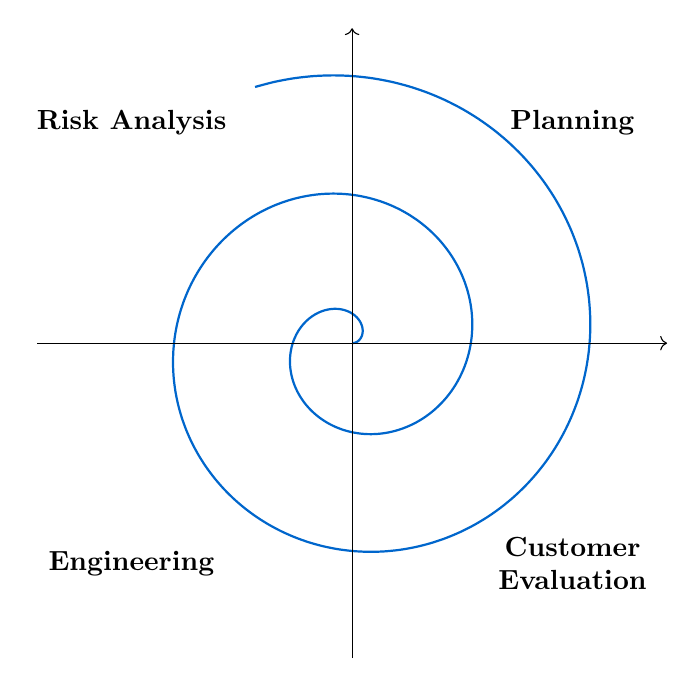
\begin{tikzpicture}[scale=0.8, auto]
    % Spiral line
    \draw [headcolor, thick, domain=0:14.5, variable=\t, samples=200, smooth] plot ({\t r}: {0.3*\t});
    
    % Axes
    \draw [->] (-5,0) -- (5,0);
    \draw [->] (0,-5) -- (0,5);
    
    % Quadrant Labels
    \node [align=center] at (3.5, 3.5) {\textbf{Planning}};
    \node [align=center] at (-3.5, 3.5) {\textbf{Risk Analysis}};
    \node [align=center] at (-3.5, -3.5) {\textbf{Engineering}};
    \node [align=center] at (3.5, -3.5) {\textbf{Customer}\\\textbf{Evaluation}};
    
\end{tikzpicture}
\captionof{figure}{Spiral Model}
\end{center}

\begin{center}
\captionof{table}{Spiral Model Phases}
\begin{tabulary}{\linewidth}{|L|L|}
\hline
\textbf{Phase} & \textbf{Activities} \\ \hline
\textbf{Planning} & Requirements gathering, resource planning \\ \hline
\textbf{Risk Analysis} & Identify and resolve risks \\ \hline
\textbf{Engineering} & Development and testing \\ \hline
\textbf{Customer Evaluation} & Customer reviews and feedback \\ \hline
\end{tabulary}
\end{center}

\textbf{Advantages}:
\begin{itemize}
    \item \textbf{Risk management}: Early risk identification
    \item \textbf{Flexibility}: Accommodates changes easily
    \item \textbf{Customer involvement}: Regular customer feedback
    \item \textbf{Quality focus}: Continuous testing and validation
\end{itemize}

\textbf{Disadvantages}:
\begin{itemize}
    \item \textbf{Complex management}: Difficult to manage
    \item \textbf{High cost}: Expensive due to risk analysis
    \item \textbf{Time consuming}: Long development cycles
    \item \textbf{Risk expertise needed}: Requires risk assessment skills
\end{itemize}

\textbf{Best for}: Large, complex, high-risk projects
\end{solutionbox}

\begin{mnemonicbox}
\mnemonic{Plan Risks Engineering Customer}
\end{mnemonicbox}

\questionmarks{2(a) OR}{3}{Explain Incremental model.}

\begin{solutionbox}
\textbf{Incremental Model} delivers software in small, functional pieces called increments.

\begin{center}
\begin{tikzpicture}[node distance=1.5cm, auto]
    \node [gtu block] (core) {Core Product};
    \node [gtu block, right of=core, xshift=1.2cm] (inc1) {Increment 1};
    \node [gtu block, right of=inc1, xshift=1.2cm] (inc2) {Increment 2};
    \node [gtu block, right of=inc2, xshift=1.2cm] (inc3) {Increment 3};
    \node [gtu block, below of=inc1, xshift=1.35cm] (final) {Final Product};
    
    \draw [gtu arrow] (core) -- (inc1);
    \draw [gtu arrow] (inc1) -- (inc2);
    \draw [gtu arrow] (inc2) -- (inc3);
    \draw [gtu arrow] (inc3) -- (final);
\end{tikzpicture}
\captionof{figure}{Incremental Delivery}
\end{center}

\textbf{Key Features}:
\begin{itemize}
    \item \textbf{Partial implementation}: Each increment adds functionality
    \item \textbf{Early delivery}: Core features delivered first
    \item \textbf{Parallel development}: Multiple increments can be developed simultaneously
\end{itemize}

\begin{center}
\captionof{table}{Incremental Model Characteristics}
\begin{tabulary}{\linewidth}{|L|L|}
\hline
\textbf{Aspect} & \textbf{Description} \\ \hline
\textbf{Delivery} & Multiple releases \\ \hline
\textbf{Functionality} & Grows with each increment \\ \hline
\textbf{Risk} & Reduced through early delivery \\ \hline
\textbf{Feedback} & Continuous user feedback \\ \hline
\end{tabulary}
\end{center}
\end{solutionbox}

\begin{mnemonicbox}
\mnemonic{Deliver Functionality Reducing Feedback}
\end{mnemonicbox}

\questionmarks{2(b) OR}{4}{Write concept of Rapid Application Development model and explain it.}

\begin{solutionbox}
\textbf{RAD (Rapid Application Development)} emphasizes rapid prototyping and quick feedback over extensive planning.

\begin{center}
\captionof{table}{RAD Model Phases}
\begin{tabulary}{\linewidth}{|L|C|L|}
\hline
\textbf{Phase} & \textbf{Duration} & \textbf{Activities} \\ \hline
\textbf{Business Modeling} & Short & Define business functions \\ \hline
\textbf{Data Modeling} & Short & Define data requirements \\ \hline
\textbf{Process Modeling} & Short & Convert data to business info \\ \hline
\textbf{Application Generation} & Short & Use tools to create software \\ \hline
\textbf{Testing \& Turnover} & Short & Test and deploy \\ \hline
\end{tabulary}
\end{center}

\textbf{Key Concepts}:
\begin{itemize}
    \item \textbf{Reusable components}: Pre-built components speed development
    \item \textbf{Powerful tools}: CASE tools and code generators
    \item \textbf{Small teams}: 2-6 people per team
    \item \textbf{Time-boxed}: Strict time limits (60-90 days)
\end{itemize}

\textbf{Requirements for RAD}:
\begin{itemize}
    \item \textbf{Well-defined business requirements}
    \item \textbf{User involvement} throughout process
    \item \textbf{Skilled developers} familiar with RAD tools
\end{itemize}
\end{solutionbox}

\begin{mnemonicbox}
\mnemonic{Business Data Process Application Testing}
\end{mnemonicbox}

\questionmarks{2(c) OR}{7}{Define SDLC and explain each phase.}

\begin{solutionbox}
\textbf{SDLC (Software Development Life Cycle)} is a systematic process for building software through well-defined phases.

\begin{center}
\begin{tikzpicture}[node distance=1.6cm, auto]
    \node [gtu state] (plan) {Planning};
    \node [gtu state, right of=plan, xshift=0.5cm] (ana) {Analysis};
    \node [gtu state, right of=ana, xshift=0.5cm] (des) {Design};
    \node [gtu state, below of=des] (imp) {Implementation};
    \node [gtu state, left of=imp, xshift=-0.5cm] (test) {Testing};
    \node [gtu state, left of=test, xshift=-0.5cm] (dep) {Deployment};
    \node [gtu state, above of=dep] (maint) {Maintenance};
    
    \draw [gtu arrow] (plan) -- (ana);
    \draw [gtu arrow] (ana) -- (des);
    \draw [gtu arrow] (des) -- (imp);
    \draw [gtu arrow] (imp) -- (test);
    \draw [gtu arrow] (test) -- (dep);
    \draw [gtu arrow] (dep) -- (maint);
    \draw [gtu arrow] (maint) -- (plan);
\end{tikzpicture}
\captionof{figure}{SDLC Cycle}
\end{center}

\begin{center}
\captionof{table}{SDLC Phases Detailed}
\begin{tabulary}{\linewidth}{|L|L|L|}
\hline
\textbf{Phase} & \textbf{Activities} & \textbf{Deliverables} \\ \hline
\textbf{Planning} & Project planning, feasibility study & Project plan \\ \hline
\textbf{Analysis} & Requirement gathering & SRS document \\ \hline
\textbf{Design} & System architecture, UI design & Design document \\ \hline
\textbf{Implementation} & Coding, unit testing & Source code \\ \hline
\textbf{Testing} & System testing, integration & Test reports \\ \hline
\textbf{Deployment} & Installation, user training & Live system \\ \hline
\textbf{Maintenance} & Bug fixes, enhancements & Updated system \\ \hline
\end{tabulary}
\end{center}

\textbf{Phase Descriptions}:
\begin{itemize}
    \item \textbf{Planning}: Define project scope and resources
    \item \textbf{Analysis}: Understand what system should do
    \item \textbf{Design}: Plan how system will work
    \item \textbf{Implementation}: Build the actual system
    \item \textbf{Testing}: Verify system works correctly
    \item \textbf{Deployment}: Release system to users
    \item \textbf{Maintenance}: Ongoing support and updates
\end{itemize}
\end{solutionbox}

\begin{mnemonicbox}
\mnemonic{People Always Design Implementation, Test Deployment, Maintain}
\end{mnemonicbox}

\questionmarks{3(a)}{3}{Describe skills to manage software projects.}

\begin{solutionbox}
\textbf{Software Project Management} requires combination of technical and soft skills.

\begin{center}
\captionof{table}{Essential Project Management Skills}
\begin{tabulary}{\linewidth}{|L|L|}
\hline
\textbf{Skill Category} & \textbf{Specific Skills} \\ \hline
\textbf{Technical} & Understanding SDLC, tools, technologies \\ \hline
\textbf{Leadership} & Team motivation, decision making \\ \hline
\textbf{Communication} & Clear communication with team and clients \\ \hline
\textbf{Planning} & Resource allocation, scheduling \\ \hline
\textbf{Problem-solving} & Risk management, conflict resolution \\ \hline
\end{tabulary}
\end{center}

\textbf{Key Skills}:
\begin{itemize}
    \item \textbf{People management}: Lead and motivate team members
    \item \textbf{Technical knowledge}: Understand development process and tools
    \item \textbf{Communication}: Bridge between technical team and stakeholders
\end{itemize}
\end{solutionbox}

\begin{mnemonicbox}
\mnemonic{Technical Leaders Communicate Planning Problems}
\end{mnemonicbox}

\questionmarks{3(b)}{4}{Briefly write responsibility of Software Project manager.}

\begin{solutionbox}
\textbf{Software Project Manager} oversees entire project from initiation to completion.

\begin{center}
\captionof{table}{Project Manager Responsibilities}
\begin{tabulary}{\linewidth}{|L|L|}
\hline
\textbf{Area} & \textbf{Responsibilities} \\ \hline
\textbf{Planning} & Create project plans, schedules, budgets \\ \hline
\textbf{Team Management} & Hire, train, and manage team members \\ \hline
\textbf{Communication} & Regular updates to stakeholders \\ \hline
\textbf{Quality Control} & Ensure deliverables meet quality standards \\ \hline
\textbf{Risk Management} & Identify and mitigate project risks \\ \hline
\end{tabulary}
\end{center}

\textbf{Primary Responsibilities}:
\begin{itemize}
    \item \textbf{Project Planning}: Define scope, timeline, and resources
    \item \textbf{Team Leadership}: Guide and support development team
    \item \textbf{Stakeholder Communication}: Keep everyone informed of progress
    \item \textbf{Quality Assurance}: Ensure project meets requirements
    \item \textbf{Risk Management}: Handle project risks and issues
\end{itemize}

\textbf{Success Factors}: On-time delivery, within budget, meeting requirements
\end{solutionbox}

\begin{mnemonicbox}
\mnemonic{Plan Team Communication Quality Risk}
\end{mnemonicbox}

\questionmarks{3(c)}{7}{Classify types of Requirements in SRS (1) Functional Requirements (2) Non-Functional Requirements.}

\begin{solutionbox}
\textbf{Requirements Classification} helps organize and understand different types of system needs.

\begin{center}
\captionof{table}{Functional vs Non-Functional Requirements}
\begin{tabulary}{\linewidth}{|L|L|L|}
\hline
\textbf{Aspect} & \textbf{Functional Requirements} & \textbf{Non-Functional Requirements} \\ \hline
\textbf{Definition} & What system should do & How system should perform \\ \hline
\textbf{Focus} & System functionality & System quality attributes \\ \hline
\textbf{Examples} & Login, search, calculate & Performance, security, usability \\ \hline
\textbf{Testing} & Functional testing & Performance testing \\ \hline
\end{tabulary}
\end{center}

\textbf{Functional Requirements}:
\begin{itemize}
    \item \textbf{User interactions}: Login, registration, data entry
    \item \textbf{Business rules}: Validation rules, calculations
    \item \textbf{System features}: Reports, notifications, workflows
    \item \textbf{Data processing}: CRUD operations
\end{itemize}

\textbf{Examples}: 
\begin{itemize}
    \item User can login with username/password
    \item System calculates tax automatically
    \item Generate monthly sales report
\end{itemize}

\textbf{Non-Functional Requirements}:

\begin{center}
\captionof{table}{Non-Functional Requirement Types}
\begin{tabulary}{\linewidth}{|L|L|L|}
\hline
\textbf{Type} & \textbf{Description} & \textbf{Example} \\ \hline
\textbf{Performance} & Speed and responsiveness & Response time < 2 seconds \\ \hline
\textbf{Security} & Data protection & Encrypted data transmission \\ \hline
\textbf{Usability} & User experience & Easy to learn interface \\ \hline
\textbf{Reliability} & System dependability & 99.9\% uptime \\ \hline
\textbf{Scalability} & Growth handling & Support 1000+ users \\ \hline
\end{tabulary}
\end{center}

\textbf{Quality Attributes}:
\begin{itemize}
    \item \textbf{Performance}: Response time, throughput
    \item \textbf{Security}: Authentication, authorization, encryption
    \item \textbf{Usability}: User-friendly interface, accessibility
    \item \textbf{Reliability}: Uptime, error handling
    \item \textbf{Maintainability}: Code quality, documentation
\end{itemize}
\end{solutionbox}

\begin{mnemonicbox}
\mnemonic{Performance Security Usability Reliability Maintainability}
\end{mnemonicbox}

\questionmarks{3(a) OR}{3}{Illustrate importance of SRS.}

\begin{solutionbox}
\textbf{SRS (Software Requirements Specification)} is crucial document that defines what software should do.

\begin{center}
\captionof{table}{SRS Importance}
\begin{tabulary}{\linewidth}{|L|L|}
\hline
\textbf{Aspect} & \textbf{Benefit} \\ \hline
\textbf{Clear Communication} & All stakeholders understand requirements \\ \hline
\textbf{Project Planning} & Basis for estimation and scheduling \\ \hline
\textbf{Quality Assurance} & Foundation for testing \\ \hline
\textbf{Change Management} & Controlled requirement changes \\ \hline
\textbf{Legal Protection} & Contract reference document \\ \hline
\end{tabulary}
\end{center}

\textbf{Key Importance}:
\begin{itemize}
    \item \textbf{Communication tool}: Bridge between clients and developers
    \item \textbf{Planning foundation}: Helps estimate time, cost, and resources
    \item \textbf{Testing basis}: Test cases derived from SRS requirements
\end{itemize}
\end{solutionbox}

\begin{mnemonicbox}
\mnemonic{Clear Planning Quality Change Legal}
\end{mnemonicbox}

\questionmarks{3(b) OR}{4}{Explain Gantt Chart.}

\begin{solutionbox}
\textbf{Gantt Chart} is a visual project management tool showing tasks, timelines, and dependencies.

\begin{center}
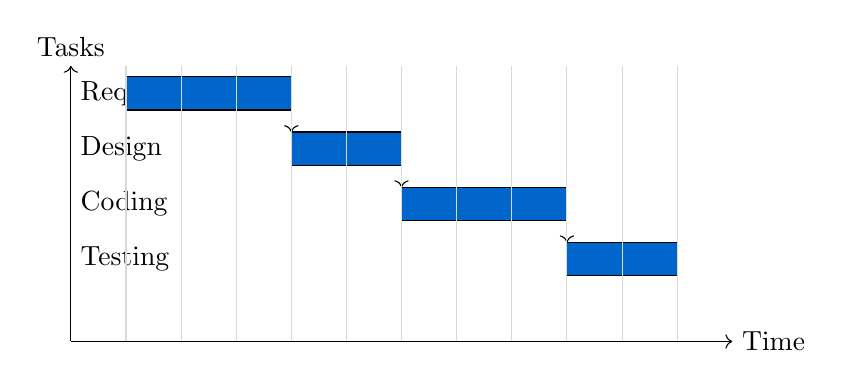
\begin{tikzpicture}[scale=0.7]
    \draw[->] (0,0) -- (12,0) node[right] {Time};
    \draw[->] (0,0) -- (0,5) node[above] {Tasks};
    
    % Tasks
    \node[right] at (0, 4.5) {Requirements};
    \draw[fill=headcolor] (1,4.2) rectangle (4,4.8);
    
    \node[right] at (0, 3.5) {Design};
    \draw[fill=headcolor] (4,3.2) rectangle (6,3.8);
    
    \node[right] at (0, 2.5) {Coding};
    \draw[fill=headcolor] (6,2.2) rectangle (9,2.8);
    
    \node[right] at (0, 1.5) {Testing};
    \draw[fill=headcolor] (9,1.2) rectangle (11,1.8);
    
    % Dependencies
    \draw[dashed, ->] (4,4.5) -- (4,3.8);
    \draw[dashed, ->] (6,3.5) -- (6,2.8);
    \draw[dashed, ->] (9,2.5) -- (9,1.8);
    
    % Grid lines (optional for visual aid)
    \foreach \x in {1,...,11} \draw[gray!30] (\x,0) -- (\x,5);
    
\end{tikzpicture}
\captionof{figure}{Simple Gantt Chart}
\end{center}

\begin{center}
\captionof{table}{Gantt Chart Components}
\begin{tabulary}{\linewidth}{|L|L|}
\hline
\textbf{Component} & \textbf{Description} \\ \hline
\textbf{Tasks} & Work items to be completed \\ \hline
\textbf{Timeline} & Horizontal time scale \\ \hline
\textbf{Bars} & Task duration and progress \\ \hline
\textbf{Dependencies} & Task relationships \\ \hline
\textbf{Milestones} & Important project events \\ \hline
\end{tabulary}
\end{center}

\textbf{Benefits}:
\begin{itemize}
    \item \textbf{Visual timeline}: Easy to see project schedule
    \item \textbf{Progress tracking}: Monitor task completion
    \item \textbf{Resource planning}: Allocate resources effectively
    \item \textbf{Dependency management}: Understand task relationships
\end{itemize}
\end{solutionbox}

\begin{mnemonicbox}
\mnemonic{Tasks Timeline Bars Dependencies Milestones}
\end{mnemonicbox}

\questionmarks{3(c) OR}{7}{Write a short note on Risk Management.}

\begin{solutionbox}
\textbf{Risk Management} is systematic process of identifying, analyzing, and controlling project risks.

\begin{center}
\begin{tikzpicture}[node distance=2.5cm, auto]
    \node [gtu state] (id) {Risk\\Identification};
    \node [gtu state, right of=id] (ana) {Risk\\Analysis};
    \node [gtu state, right of=ana] (plan) {Risk\\Planning};
    \node [gtu state, right of=plan] (mon) {Risk\\Monitoring};

    \draw [gtu arrow] (id) -- (ana);
    \draw [gtu arrow] (ana) -- (plan);
    \draw [gtu arrow] (plan) -- (mon);
    \draw [gtu arrow] (mon)edge [bend left=30] (id);
\end{tikzpicture}
\captionof{figure}{Risk Management Cycle}
\end{center}

\begin{center}
\captionof{table}{Risk Management Process}
\begin{tabulary}{\linewidth}{|L|L|L|}
\hline
\textbf{Phase} & \textbf{Activities} & \textbf{Output} \\ \hline
\textbf{Identification} & Find potential risks & Risk list \\ \hline
\textbf{Analysis} & Assess probability and impact & Risk priority \\ \hline
\textbf{Planning} & Develop response strategies & Risk response plan \\ \hline
\textbf{Monitoring} & Track and control risks & Updated risk status \\ \hline
\end{tabulary}
\end{center}

\textbf{Risk Categories}:

\begin{center}
\captionof{table}{Types of Software Risks}
\begin{tabulary}{\linewidth}{|L|L|}
\hline
\textbf{Category} & \textbf{Examples} \\ \hline
\textbf{Technical} & Technology changes, complexity \\ \hline
\textbf{Project} & Schedule delays, resource shortage \\ \hline
\textbf{Business} & Market changes, funding issues \\ \hline
\textbf{External} & Vendor problems, regulatory changes \\ \hline
\end{tabulary}
\end{center}

\textbf{Risk Response Strategies}:
\begin{itemize}
    \item \textbf{Avoid}: Eliminate risk source
    \item \textbf{Mitigate}: Reduce probability or impact  
    \item \textbf{Transfer}: Share risk with others
    \item \textbf{Accept}: Live with the risk
\end{itemize}

\textbf{Risk Assessment}: Probability $\times$ Impact = Risk Exposure

\textbf{Benefits}: Proactive problem solving, better project success rate, stakeholder confidence
\end{solutionbox}

\begin{mnemonicbox}
\mnemonic{Identify Analyze Plan Monitor (Process), Avoid Mitigate Transfer Accept (Strategies)}
\end{mnemonicbox}

\questionmarks{4(a)}{3}{What is metric for size estimation? Explain FP with example.}

\begin{solutionbox}
\textbf{Size Estimation Metrics} help predict software project size and effort.

\begin{center}
\captionof{table}{Size Estimation Metrics}
\begin{tabulary}{\linewidth}{|L|L|}
\hline
\textbf{Metric} & \textbf{Description} \\ \hline
\textbf{LOC} & Lines of Code \\ \hline
\textbf{Function Points} & Functionality-based measurement \\ \hline
\textbf{Object Points} & For object-oriented systems \\ \hline
\textbf{Feature Points} & Enhanced function points \\ \hline
\end{tabulary}
\end{center}

\textbf{Function Points (FP)} measure software size based on user functionality.

\textbf{FP Components}:
\begin{itemize}
    \item \textbf{External Inputs}: Data entry screens
    \item \textbf{External Outputs}: Reports, messages  
    \item \textbf{External Queries}: Database queries
    \item \textbf{Internal Files}: Data stores
    \item \textbf{External Interfaces}: System connections
\end{itemize}

\textbf{FP Calculation Example}:
For a Library Management System:
\begin{itemize}
    \item External Inputs: 5 (Book entry, Member entry, etc.)
    \item External Outputs: 3 (Reports)
    \item External Queries: 4 (Search functions)
    \item Internal Files: 2 (Book DB, Member DB)
    \item External Interfaces: 1 (Online catalog)
\end{itemize}

\textbf{Simple FP = 5 + 3 + 4 + 2 + 1 = 15 Function Points}
\end{solutionbox}

\begin{mnemonicbox}
\mnemonic{Inputs Outputs Queries Files Interfaces}
\end{mnemonicbox}

\questionmarks{4(b)}{4}{Explain project estimation techniques using basic COCOMO model.}

\begin{solutionbox}
\textbf{COCOMO (COnstructive COst MOdel)} estimates software development effort and schedule.

\begin{center}
\captionof{table}{COCOMO Model Types}
\begin{tabulary}{\linewidth}{|L|L|L|}
\hline
\textbf{Type} & \textbf{Description} & \textbf{Accuracy} \\ \hline
\textbf{Basic} & Simple size-based estimation & $\pm$75\% \\ \hline
\textbf{Intermediate} & Includes cost drivers & $\pm$25\% \\ \hline
\textbf{Detailed} & Phase-level estimation & $\pm$10\% \\ \hline
\end{tabulary}
\end{center}

\textbf{Basic COCOMO Formula}:
\begin{itemize}
    \item \textbf{Effort} = $a \times (KLOC)^b$ person-months
    \item \textbf{Time} = $c \times (Effort)^d$ months
    \item \textbf{People} = Effort / Time
\end{itemize}

\begin{center}
\captionof{table}{COCOMO Constants}
\begin{tabulary}{\linewidth}{|L|C|C|C|C|}
\hline
\textbf{Project Type} & \textbf{a} & \textbf{b} & \textbf{c} & \textbf{d} \\ \hline
\textbf{Organic} & 2.4 & 1.05 & 2.5 & 0.38 \\ \hline
\textbf{Semi-detached} & 3.0 & 1.12 & 2.5 & 0.35 \\ \hline
\textbf{Embedded} & 3.6 & 1.20 & 2.5 & 0.32 \\ \hline
\end{tabulary}
\end{center}

\textbf{Example}: For 10 KLOC organic project
\begin{itemize}
    \item Effort = $2.4 \times (10)^{1.05} = 25.47$ person-months
    \item Time = $2.5 \times (25.47)^{0.38} = 8.64$ months
    \item People = $25.47 / 8.64 = 3$ people
\end{itemize}
\end{solutionbox}

\begin{mnemonicbox}
\mnemonic{Organic Semi Embedded}
\end{mnemonicbox}

\questionmarks{4(c)}{7}{Prepare Sprint burn down chart for system of your choice.}

\begin{solutionbox}
\textbf{Sprint Burn Down Chart} tracks remaining work during a sprint for \textbf{Online Shopping System}.

\textbf{Sprint Goal}: User Authentication Module (40 Story Points, 2 Weeks Estimate)

\begin{center}
\begin{tikzpicture}[scale=0.8]
    % Axes
    \draw[->] (0,0) -- (11,0) node[right] {Day};
    \draw[->] (0,0) -- (0,9) node[above] {Story Points};
    
    % Y-axis labels
    \foreach \y/\label in {0/0, 2/10, 4/20, 6/30, 8/40}
        \node at (-0.5,\y) {\label};
    
    % X-axis labels
    \foreach \x/\label in {1/2, 2/4, 3/6, 4/8, 5/10, 6/12, 7/14}
        \node at (\x*1.4,-0.5) {\label};
    
    % Ideal line
    \draw[dashed, thick] (0,8) -- (10,0);
    
    % Actual progress
    \draw[thick, headcolor] (0,8) -- (1.4,7.6) -- (2.8,7) -- (4.2,6.4) -- (5.6,5.4) -- (7,5.0) -- (8.4,4) -- (10,0);
    
    % Legend
    \node[right] at (8,8) {Ideal};
    \node[right, headcolor] at (8,7.5) {Actual};
\end{tikzpicture}
\captionof{figure}{Sprint Burn Down Chart}
\end{center}

\textbf{Sprint Backlog}:

\begin{center}
\captionof{table}{Sprint Tasks}
\begin{tabulary}{\linewidth}{|L|C|L|}
\hline
\textbf{Task} & \textbf{Story Points} & \textbf{Day Assigned} \\ \hline
\textbf{User Registration} & 8 & Day 1-2 \\ \hline
\textbf{User Login} & 6 & Day 3-4 \\ \hline
\textbf{Password Reset} & 5 & Day 5-6 \\ \hline
\textbf{Profile Management} & 8 & Day 7-8 \\ \hline
\textbf{Session Management} & 6 & Day 9-10 \\ \hline
\textbf{Testing \& Bug Fixes} & 7 & Day 11-14 \\ \hline
\end{tabulary}
\end{center}

\textbf{Burn Down Chart Data}:

\begin{center}
\captionof{table}{Daily Progress}
\begin{tabulary}{\linewidth}{|L|C|C|L|}
\hline
\textbf{Day} & \textbf{Ideal} & \textbf{Actual} & \textbf{Status} \\ \hline
\textbf{Day 0} & 40 & 40 & Sprint Start \\ \hline
\textbf{Day 2} & 36 & 38 & Registration delay \\ \hline
\textbf{Day 4} & 32 & 32 & Login completed \\ \hline
\textbf{Day 6} & 28 & 27 & Password reset done \\ \hline
\textbf{Day 8} & 24 & 26 & Profile issues \\ \hline
\textbf{Day 10} & 20 & 20 & Back on track \\ \hline
\textbf{Day 12} & 16 & 15 & Testing well \\ \hline
\textbf{Day 14} & 0 & 0 & Completed \\ \hline
\end{tabulary}
\end{center}

\textbf{Chart Analysis}:
\begin{itemize}
    \item \textbf{Green line}: Ideal burn down
    \item \textbf{Red line}: Actual progress  
    \item \textbf{Variations}: Show challenges and recoveries
    \item \textbf{Completion}: Sprint finished on time
\end{itemize}

\textbf{Benefits}: Visual progress tracking, early problem identification, team motivation
\end{solutionbox}

\begin{mnemonicbox}
\mnemonic{Track Progress Daily, Identify Issues Early}
\end{mnemonicbox}

\questionmarks{4(a) OR}{3}{Explain the component of USE CASE diagram.}

\begin{solutionbox}
\textbf{Use Case Diagram} shows system functionality from user perspective.

\begin{center}
\captionof{table}{Use Case Diagram Components}
\begin{tabulary}{\linewidth}{|L|C|L|}
\hline
\textbf{Component} & \textbf{Symbol} & \textbf{Description} \\ \hline
\textbf{Actor} & Stick figure & External entity interacting with system \\ \hline
\textbf{Use Case} & Oval & System functionality \\ \hline
\textbf{System Boundary} & Rectangle & System scope \\ \hline
\textbf{Association} & Line & Actor-Use Case relationship \\ \hline
\textbf{Generalization} & Arrow & Inheritance relationship \\ \hline
\end{tabulary}
\end{center}

\textbf{Relationships}:
\begin{itemize}
    \item \textbf{Include}: One use case includes another (mandatory)
    \item \textbf{Extend}: Optional use case extension
    \item \textbf{Generalization}: Parent-child relationship
\end{itemize}

\textbf{Example Components}:
\begin{itemize}
    \item \textbf{Primary Actor}: Customer, Admin
    \item \textbf{Use Cases}: Login, Search Products, Place Order
    \item \textbf{System}: Online Shopping System
\end{itemize}
\end{solutionbox}

\begin{mnemonicbox}
\mnemonic{Actors Use Systems, Associate Generally}
\end{mnemonicbox}

\questionmarks{4(b) OR}{4}{Compare Cohesion and Coupling.}

\begin{solutionbox}
\textbf{Cohesion and Coupling} are important software design principles affecting maintainability.

\begin{center}
\captionof{table}{Cohesion vs Coupling Comparison}
\begin{tabulary}{\linewidth}{|L|L|L|}
\hline
\textbf{Aspect} & \textbf{Cohesion} & \textbf{Coupling} \\ \hline
\textbf{Definition} & Unity within module & Dependency between modules \\ \hline
\textbf{Desirable Level} & High cohesion preferred & Low coupling preferred \\ \hline
\textbf{Focus} & Internal module unity & Inter-module relationships \\ \hline
\textbf{Impact} & Module reliability & System flexibility \\ \hline
\textbf{Measurement} & How related are module elements & How dependent modules are \\ \hline
\end{tabulary}
\end{center}

\textbf{Cohesion Types} (Low to High):
\begin{itemize}
    \item \textbf{Coincidental, Logical, Temporal, Procedural, Communicational, Sequential, Functional}
\end{itemize}

\textbf{Coupling Types} (High to Low):
\begin{itemize}
    \item \textbf{Content, Common, External, Control, Stamp, Data}
\end{itemize}

\textbf{Goal}: \textbf{High Cohesion + Low Coupling = Good Design}
\end{solutionbox}

\begin{mnemonicbox}
\mnemonic{High Cohesion, Low Coupling}
\end{mnemonicbox}

\questionmarks{4(c) OR}{7}{Explain Risk Assessment in detail.}

\begin{solutionbox}
\textbf{Risk Assessment} evaluates identified risks to prioritize management efforts.

\begin{center}
\begin{tikzpicture}[node distance=2cm, auto]
    \node [gtu block] (id) {Risk Identification};
    \node [gtu block, right of=id, xshift=1.5cm] (assess) {Risk Assessment};
    
    \node [gtu state, below of=assess, xshift=-1.5cm] (prob) {Probability Analysis};
    \node [gtu state, below of=assess, xshift=1.5cm] (imp) {Impact Analysis};
    
    \node [gtu block, below of=assess, yshift=-2cm] (exp) {Risk Exposure};
    \node [gtu block, below of=exp] (prio) {Risk Prioritization};
    
    \draw [gtu arrow] (id) -- (assess);
    \draw [gtu arrow] (assess) -- (prob);
    \draw [gtu arrow] (assess) -- (imp);
    \draw [gtu arrow] (prob) -- (exp);
    \draw [gtu arrow] (imp) -- (exp);
    \draw [gtu arrow] (exp) -- (prio);
\end{tikzpicture}
\captionof{figure}{Risk Assessment Process}
\end{center}

\begin{center}
\captionof{table}{Risk Assessment Elements}
\begin{tabulary}{\linewidth}{|L|L|L|}
\hline
\textbf{Element} & \textbf{Description} & \textbf{Scale} \\ \hline
\textbf{Probability} & Likelihood of risk occurring & 0.1 to 1.0 \\ \hline
\textbf{Impact} & Consequences if risk occurs & 1 to 10 \\ \hline
\textbf{Risk Exposure} & Probability $\times$ Impact & Calculated value \\ \hline
\textbf{Risk Level} & Priority classification & High/Medium/Low \\ \hline
\end{tabulary}
\end{center}

\textbf{Assessment Process}:

\textbf{1. Probability Assessment}:
\begin{itemize}
    \item \textbf{Very Low (0.1) - Very High (0.9)}: Likelihood scale
\end{itemize}

\textbf{2. Impact Assessment}:
\begin{itemize}
    \item \textbf{Catastrophic (9-10)} to \textbf{Negligible (1-3)}: Consequence scale
\end{itemize}

\textbf{3. Risk Exposure Calculation}:
\textbf{Risk Exposure = Probability $\times$ Impact}

\textbf{Example Risk Assessment}:

\begin{center}
\captionof{table}{Sample Risk Analysis}
\begin{tabulary}{\linewidth}{|L|C|C|C|L|}
\hline
\textbf{Risk} & \textbf{Prob} & \textbf{Imp} & \textbf{Exp} & \textbf{Priority} \\ \hline
\textbf{Key developer leaves} & 0.3 & 8 & 2.4 & Medium \\ \hline
\textbf{Requirements change} & 0.7 & 6 & 4.2 & High \\ \hline
\textbf{Technology failure} & 0.2 & 9 & 1.8 & Low \\ \hline
\textbf{Budget cuts} & 0.4 & 7 & 2.8 & Medium \\ \hline
\end{tabulary}
\end{center}

\textbf{Risk Matrix}:
\begin{itemize}
    \item \textbf{High}: Exposure > 4.0 | \textbf{Medium}: 2.0-4.0 | \textbf{Low}: < 2.0
\end{itemize}
\end{solutionbox}

\begin{mnemonicbox}
\mnemonic{Probability Impact Exposure Priority}
\end{mnemonicbox}

\questionmarks{5(a)}{3}{Explain code inspection technique in code review.}

\begin{solutionbox}
\textbf{Code Inspection} is formal, systematic examination of code to find defects.

\begin{center}
\captionof{table}{Code Inspection Process}
\begin{tabulary}{\linewidth}{|L|L|L|}
\hline
\textbf{Phase} & \textbf{Participants} & \textbf{Activities} \\ \hline
\textbf{Planning} & Moderator & Schedule, distribute code \\ \hline
\textbf{Overview} & Author, Team & Author explains code \\ \hline
\textbf{Preparation} & Individual & Reviewers study code \\ \hline
\textbf{Inspection} & All reviewers & Find defects \\ \hline
\textbf{Rework} & Author & Fix defects \\ \hline
\textbf{Follow-up} & Moderator & Verify fixes \\ \hline
\end{tabulary}
\end{center}

\textbf{Key Features}:
\begin{itemize}
    \item \textbf{Formal process}: Structured approach with defined roles
    \item \textbf{Systematic review}: Line-by-line examination
    \item \textbf{Defect focused}: Find errors, not solutions
    \item \textbf{No author criticism}: Focus on code, not coder
\end{itemize}
\end{solutionbox}

\begin{mnemonicbox}
\mnemonic{Plan Overview Prepare Inspect Rework Follow-up}
\end{mnemonicbox}

\questionmarks{5(b)}{4}{Prepare at least four test cases of ATM.}

\begin{solutionbox}
\textbf{ATM Test Cases} verify automated teller machine functionality.

\begin{center}
\captionof{table}{ATM Test Cases}
\begin{tabulary}{\linewidth}{|L|L|L|L|L|}
\hline
\textbf{ID} & \textbf{Scenario} & \textbf{Input} & \textbf{Output} & \textbf{Result} \\ \hline
\textbf{TC1} & Valid PIN & Correct PIN & Access granted & Pass \\ \hline
\textbf{TC2} & Invalid PIN & Wrong PIN & Card blocked & Pass \\ \hline
\textbf{TC3} & Withdrawal & Amt $\le$ Bal & Cash dispensed & Pass \\ \hline
\textbf{TC4} & Low Balance & Amt $>$ Bal & Declined & Pass \\ \hline
\end{tabulary}
\end{center}

\textbf{Detailed Test Cases}:
\begin{itemize}
    \item \textbf{Valid Login}: Pre: Card inserted. Action: Enter PIN. Exp: Menu.
    \item \textbf{Cash Withdrawal}: Pre: Logged in. Action: Enter amount. Exp: Cash + Receipt.
    \item \textbf{Balance Inquiry}: Action: Check Balance. Exp: Show Balance.
    \item \textbf{PIN Change}: Action: Enter old/new PIN. Exp: Updated PIN.
\end{itemize}
\end{solutionbox}

\begin{mnemonicbox}
\mnemonic{Login Withdraw Inquiry Change}
\end{mnemonicbox}

\questionmarks{5(c)}{7}{Describe white box testing.}

\begin{solutionbox}
\textbf{White Box Testing} examines internal code structure and logic paths.

\begin{center}
\begin{tikzpicture}[node distance=1.5cm, auto]
    \node [gtu block] (code) {Source Code};
    \node [gtu block, right of=code, xshift=1cm] (cf) {Control Flow};
    \node [gtu block, right of=cf, xshift=1cm] (path) {Path Coverage};
    \node [gtu block, below of=code] (design) {Test Design};
    \node [gtu block, below of=cf] (exec) {Execution};
    \node [gtu block, below of=path] (anl) {Coverage Analysis};
    
    \draw [gtu arrow] (code) -- (cf);
    \draw [gtu arrow] (cf) -- (path);
    \draw [gtu arrow] (path) -- (design);
    \draw [gtu arrow] (design) -- (exec);
    \draw [gtu arrow] (exec) -- (anl);
\end{tikzpicture}
\captionof{figure}{White Box Testing Process}
\end{center}

\begin{center}
\captionof{table}{White Box Testing Characteristics}
\begin{tabulary}{\linewidth}{|L|L|}
\hline
\textbf{Aspect} & \textbf{Description} \\ \hline
\textbf{Focus} & Internal code structure \\ \hline
\textbf{Knowledge} & Code implementation details \\ \hline
\textbf{Coverage} & Statements, branches, paths \\ \hline
\textbf{Techniques} & Basis path, loop testing \\ \hline
\end{tabulary}
\end{center}

\textbf{Coverage Criteria}:
\begin{itemize}
    \item \textbf{Statement Coverage}: Execute every statement
    \item \textbf{Branch Coverage}: Execute all if-else paths
    \item \textbf{Path Coverage}: Execute every possible path
    \item \textbf{Condition Coverage}: Test all conditions (true/false)
\end{itemize}

\textbf{Techniques}:
\begin{enumerate}
    \item \textbf{Basis Path Testing}:
    \begin{itemize}
        \item Cyclomatic Complexity $V(G) = E - N + 2$
        \item Generate independent paths equal to $V(G)$
    \end{itemize}
    \item \textbf{Loop Testing}: Simple, Nested, Concatenated loops.
    \item \textbf{Condition Testing}: Test logical conditions.
\end{enumerate}

\textbf{Example Code}:
\begin{lstlisting}[language=C]
if (age >= 18 && income > 25000)
    approve_loan();
else
    reject_loan();
\end{lstlisting}

\textbf{Test Cases}:
\begin{itemize}
    \item age=20, income=30000 (Both True) $\to$ Approve
    \item age=16, income=30000 (First False) $\to$ Reject
    \item age=20, income=20000 (Second False) $\to$ Reject
    \item age=16, income=20000 (Both False) $\to$ Reject
\end{itemize}

\textbf{Advantages}: Thorough testing, Finds logic errors, Coverage measurement \\
\textbf{Disadvantages}: Time consuming, Expensive, Code dependent
\end{solutionbox}

\begin{mnemonicbox}
\mnemonic{Statement Branch Path Condition}
\end{mnemonicbox}

\questionmarks{5(a) OR}{3}{Explain code walk through Technique in code review.}

\begin{solutionbox}
\textbf{Code Walk Through} is informal code review technique where author presents code to team.

\begin{center}
\captionof{table}{Walk Through Process}
\begin{tabulary}{\linewidth}{|L|L|L|}
\hline
\textbf{Phase} & \textbf{Description} & \textbf{Duration} \\ \hline
\textbf{Preparation} & Author prepares presentation & 30 min \\ \hline
\textbf{Presentation} & Author explains code logic & 1-2 hours \\ \hline
\textbf{Discussion} & Team asks questions & 30 min \\ \hline
\textbf{Documentation} & Record issues & 15 min \\ \hline
\end{tabulary}
\end{center}

\textbf{Key Characteristics}:
\begin{itemize}
    \item \textbf{Author-led}: Code author drives the session
    \item \textbf{Informal process}: Less structured than inspection
    \item \textbf{Educational}: Team learns about code functionality
    \item \textbf{Collaborative}: Open discussion encouraged
\end{itemize}

\textbf{Participants}: Author (Presents), Reviewers (Ask questions), Moderator (Optional)
\end{solutionbox}

\begin{mnemonicbox}
\mnemonic{Prepare Present Discuss Document}
\end{mnemonicbox}

\questionmarks{5(b) OR}{4}{Explain software documentation.}

\begin{solutionbox}
\textbf{Software Documentation} provides information about software system for various stakeholders.

\begin{center}
\captionof{table}{Documentation Types}
\begin{tabulary}{\linewidth}{|L|L|L|}
\hline
\textbf{Type} & \textbf{Purpose} & \textbf{Audience} \\ \hline
\textbf{User Doc} & How to use software & End users \\ \hline
\textbf{System Doc} & Technical details & Developers \\ \hline
\textbf{Process Doc} & Development process & Project team \\ \hline
\textbf{Requirements} & What system should do & Stakeholders \\ \hline
\end{tabulary}
\end{center}

\textbf{Internal Documentation}: Code comments, Function headers, Variable names, README.

\textbf{External Documentation}: User manuals, Installation guides, API docs, Training materials.

\textbf{Benefits}: Maintainability, Knowledge transfer, User support, Quality assurance.
\end{solutionbox}

\begin{mnemonicbox}
\mnemonic{User System Process Requirements}
\end{mnemonicbox}

\questionmarks{5(c) OR}{7}{Write a short note on black box testing.}

\begin{solutionbox}
\textbf{Black Box Testing} examines software functionality without knowledge of internal code structure.

\begin{center}
\begin{tikzpicture}[node distance=1.5cm, auto]
    \node [gtu block] (input) {Input};
    \node [gtu block, right of=input, xshift=1.5cm, fill=black!80, text=white] (bb) {Black Box\\System};
    \node [gtu block, right of=bb, xshift=1.5cm] (output) {Output};
    
    \node [gtu state, below of=input] (tc) {Test Cases};
    \node [gtu state, below of=output] (exp) {Expected};
    \node [gtu block, below of=bb] (compare) {Compare};
    
    \draw [gtu arrow] (input) -- (bb);
    \draw [gtu arrow] (bb) -- (output);
    \draw [gtu arrow] (tc) -- (input);
    \draw [gtu arrow] (exp) -- (compare);
    \draw [gtu arrow] (output) -- (compare);
\end{tikzpicture}
\captionof{figure}{Black Box Testing Concept}
\end{center}

\begin{center}
\captionof{table}{Testing Techniques}
\begin{tabulary}{\linewidth}{|L|L|L|}
\hline
\textbf{Technique} & \textbf{Description} & \textbf{Example} \\ \hline
\textbf{Equivalence Partitioning} & Valid/Invalid classes & Age: 0-17, 18-65, >65 \\ \hline
\textbf{Boundary Value} & Test at boundaries & Age: 17, 18, 65, 66 \\ \hline
\textbf{Decision Table} & Complex rules & Insurance premium \\ \hline
\textbf{State Transition} & State changes & ATM states \\ \hline
\end{tabulary}
\end{center}

\textbf{Techniques Detail}:
\begin{enumerate}
    \item \textbf{Equivalence Partitioning}: Test one value from each partition (Valid/Invalid).
    \item \textbf{Boundary Value Analysis}: Test min, max, min-1, max+1.
    \item \textbf{Decision Table}: Mapping conditions to actions.
\end{enumerate}

\textbf{Comparison}:
\begin{itemize}
    \item \textbf{User perspective} vs Code perspective
    \item \textbf{No code knowledge needed} vs Programming skills
    \item \textbf{Early testing} vs Testing after code
\end{itemize}

\textbf{Types}: Functional, Non-functional, Regression, UAT.
\end{solutionbox}

\begin{mnemonicbox}
\mnemonic{Equivalence Boundary Decision State}
\end{mnemonicbox}

\end{document}
